%
% File: chap01.tex
% Author: Victor F. Brena-Medina
% Description: Introduction chapter where the biology goes.
%
\let\textcircled=\pgftextcircled
\chapter{Architecture}
\label{chap3}
\initial{T}his project focuses on two-person human-human interaction classification and detection in videos. Almost all of the few previous works \cite{patron2010} \cite{narayan2014} \cite{choi2012} of the two-person human-human interaction recognition adopt hand-crafted feature descriptors. For example, Narayan et al. \cite{narayan2014} combine improved trajectory features and the foreground motion map features in order to present interaction features while Patron-Perez et al. \cite{patron2010} and Choi et al. \cite{choi2012} use a hierarchical model to present interaction features. In the hierarchical model,  each individual is tracked throughout the videos, and the atomic activity for each individual and their relative position and orientations are computed first and then the collective interaction is represented. Our work adopts the hierarchical model similar to \cite{patron2010} but we replace the hand-crafted feature descriptors with the deep learning feature descriptors since deep learning based methods \cite{Ji2013} \cite{Tran2015} \cite{simonyan2014} \cite{Ng2015} have already achieved better performance in the related domains, such as single person action recognitions in videos, than hand-crafted feature descriptors\cite{grepory2010} \cite{alex2008} \cite{paul2007} \cite{wang2012} \cite{wang2013}. 
    
\section{Overall Framework}
\label{3_1}
Since we define two tasks including interaction classification and detection in our project and we set the classification as the basis for the detection, we will first introduce the overall framework of the interaction classification followed by the introduction of the architecture of the interaction detection.
\subsection{Interaction classification} 
\label{arch_classification}
Due to lack of sufficient large-scale two-person interaction datasets to just train a single deep learning network, we adopt the hierarchical model similar to \cite{choi2012} and  \cite{patron2010} which learn atomic action features for each individual in the video and concatenate these features to represent the collective interaction features. In contrast to  \cite{choi2012} and \cite{patron2010} which adopt hand-crafted features descriptors, such as HOG \cite{hog} and BoV \cite{bov}, we employ the deep learning networks as the feature descriptors.
\par    
The overall framework of our interaction classifier is illustrated in Figure \ref{fig:arch_classification}. In our architecture, we first apply the person detection to locate and track the position of each person in the input segmented videos of the UT-Interaction dataset, see Section \ref{ut-interaction}, and then crop each video into two video segments, each of which contains one person's activity. Then we design an atomic action spatial-temporal feature descriptor for each person. Since there are lots of large scale single person action datasets available, we can pre-train the atomic action feature descriptors with those datasets, such as \textbf{the ucf101 action dataset} \cite{ucf101}, and finetune the parameters on our target interaction dataset.
\par 
One drawback of this hierarchical model is that it ignore the important relative information between the two people, such as their relative position and orientation, etc. To fix this, we introduce another global feature descriptor to learn those relative information which can be trained directly on our target dataset \textbf{UT-Interaction}. 
\par 
The features extracted by the global interaction feature descriptor (\(F_g\)) and the features extracted by the atomic action feature descriptors (\(F_{a0}\) and \(F_{a1}\)) are concatenated and fed to the Classifier.  
 
 \begin{figure}
 	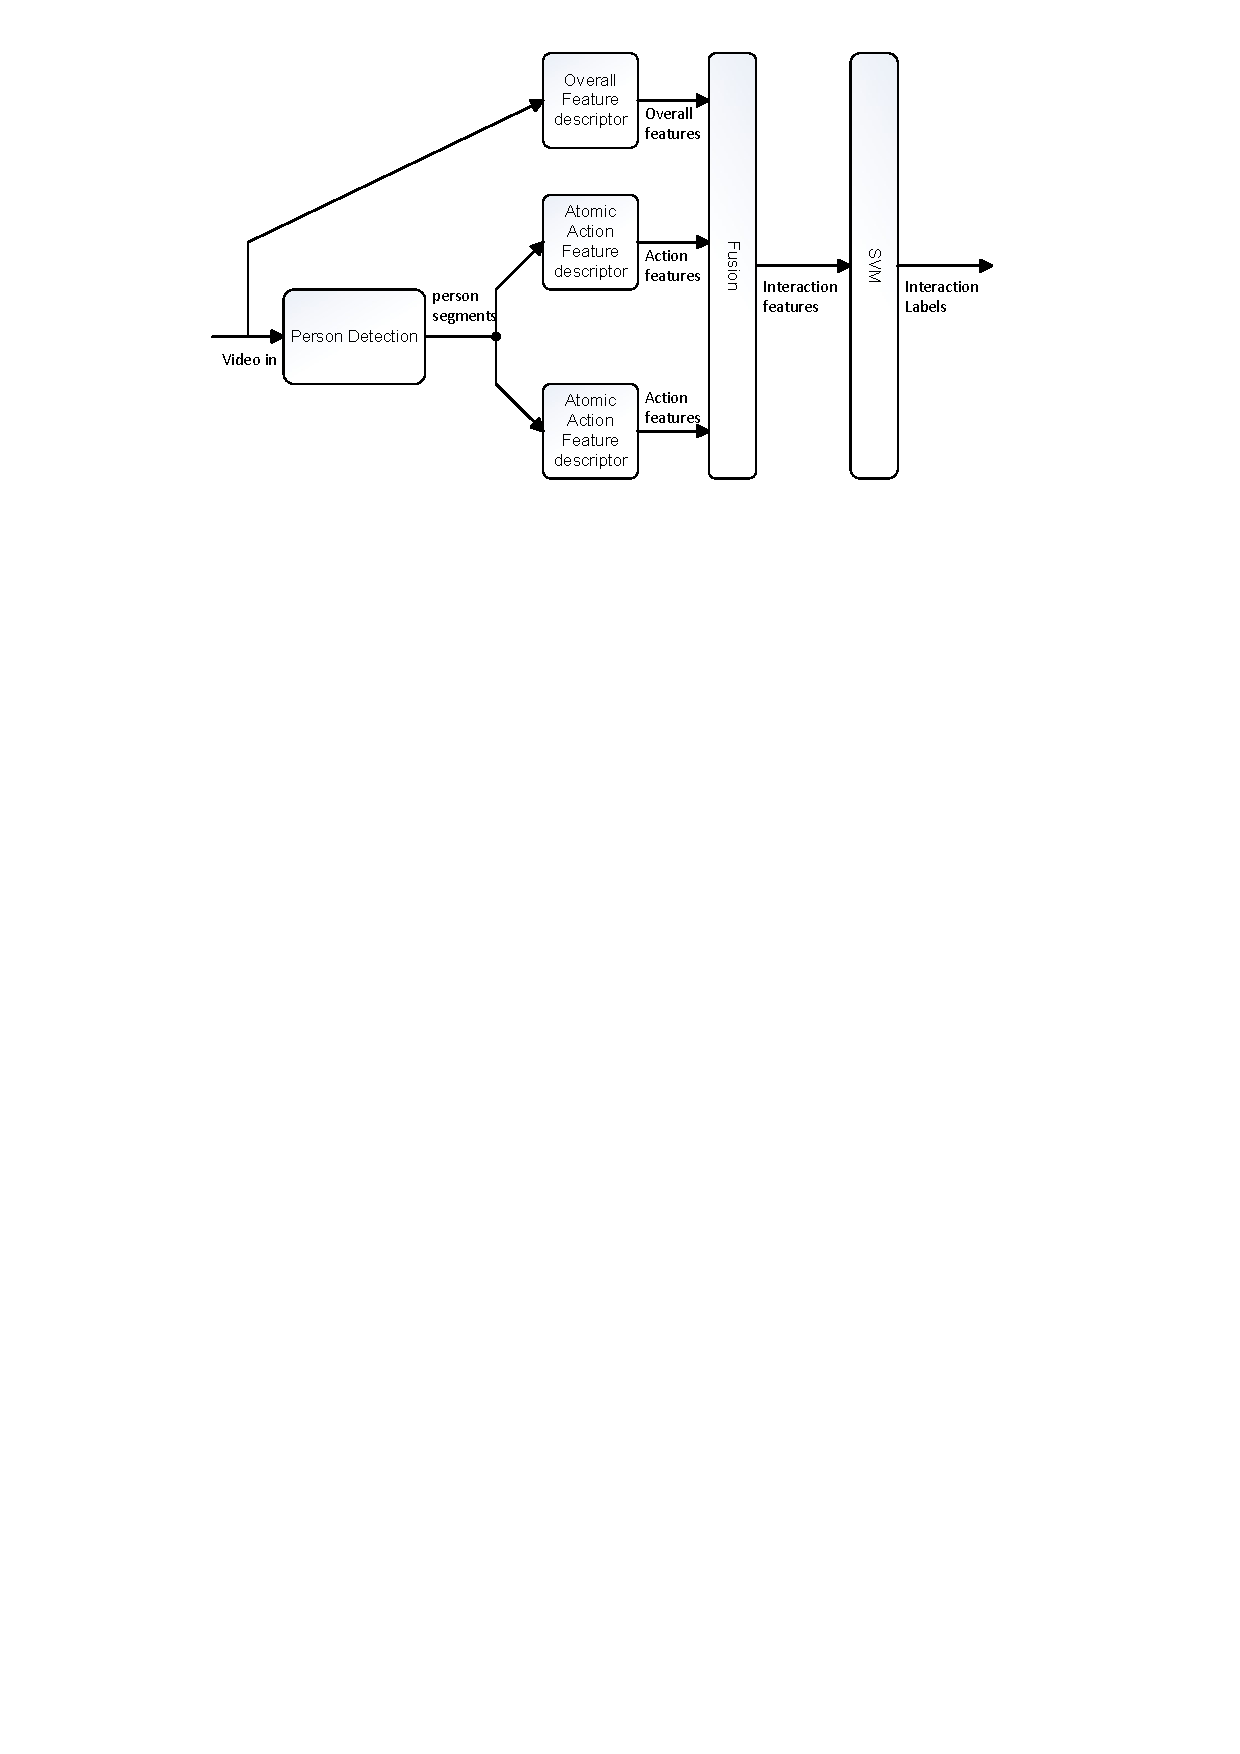
\includegraphics[trim=2cm 21.5cm 0cm 1cm]{fig01/architecture.pdf}
 	\caption{Overall framework of the interaction classification. }
 	\label{fig:arch_classification}
 \end{figure}

\subsection{Interaction detection}
The overall architecture of the interaction detection is illustrated in Figure \ref{fig:arch_det}. We first perform the spatial detection of interacting people followed by the temporal detection of interaction instead of directly applying a spatial-temporal variable size sliding window. Because the later one costs lots of computation resources and is very timing consuming. We define the spatial detection of interacting people as spatially locating the interacting people in each frame and tracking them throughout the video. Then we can make use of these spatial locations of the interacting people to generate candidate video clips by temporally sliding a 3D (\(x,y,t\)) window. Then we apply temporal detection of interactions based on the interaction classification model defined in the Section \ref{arch_classification}.       
 \begin{figure}
	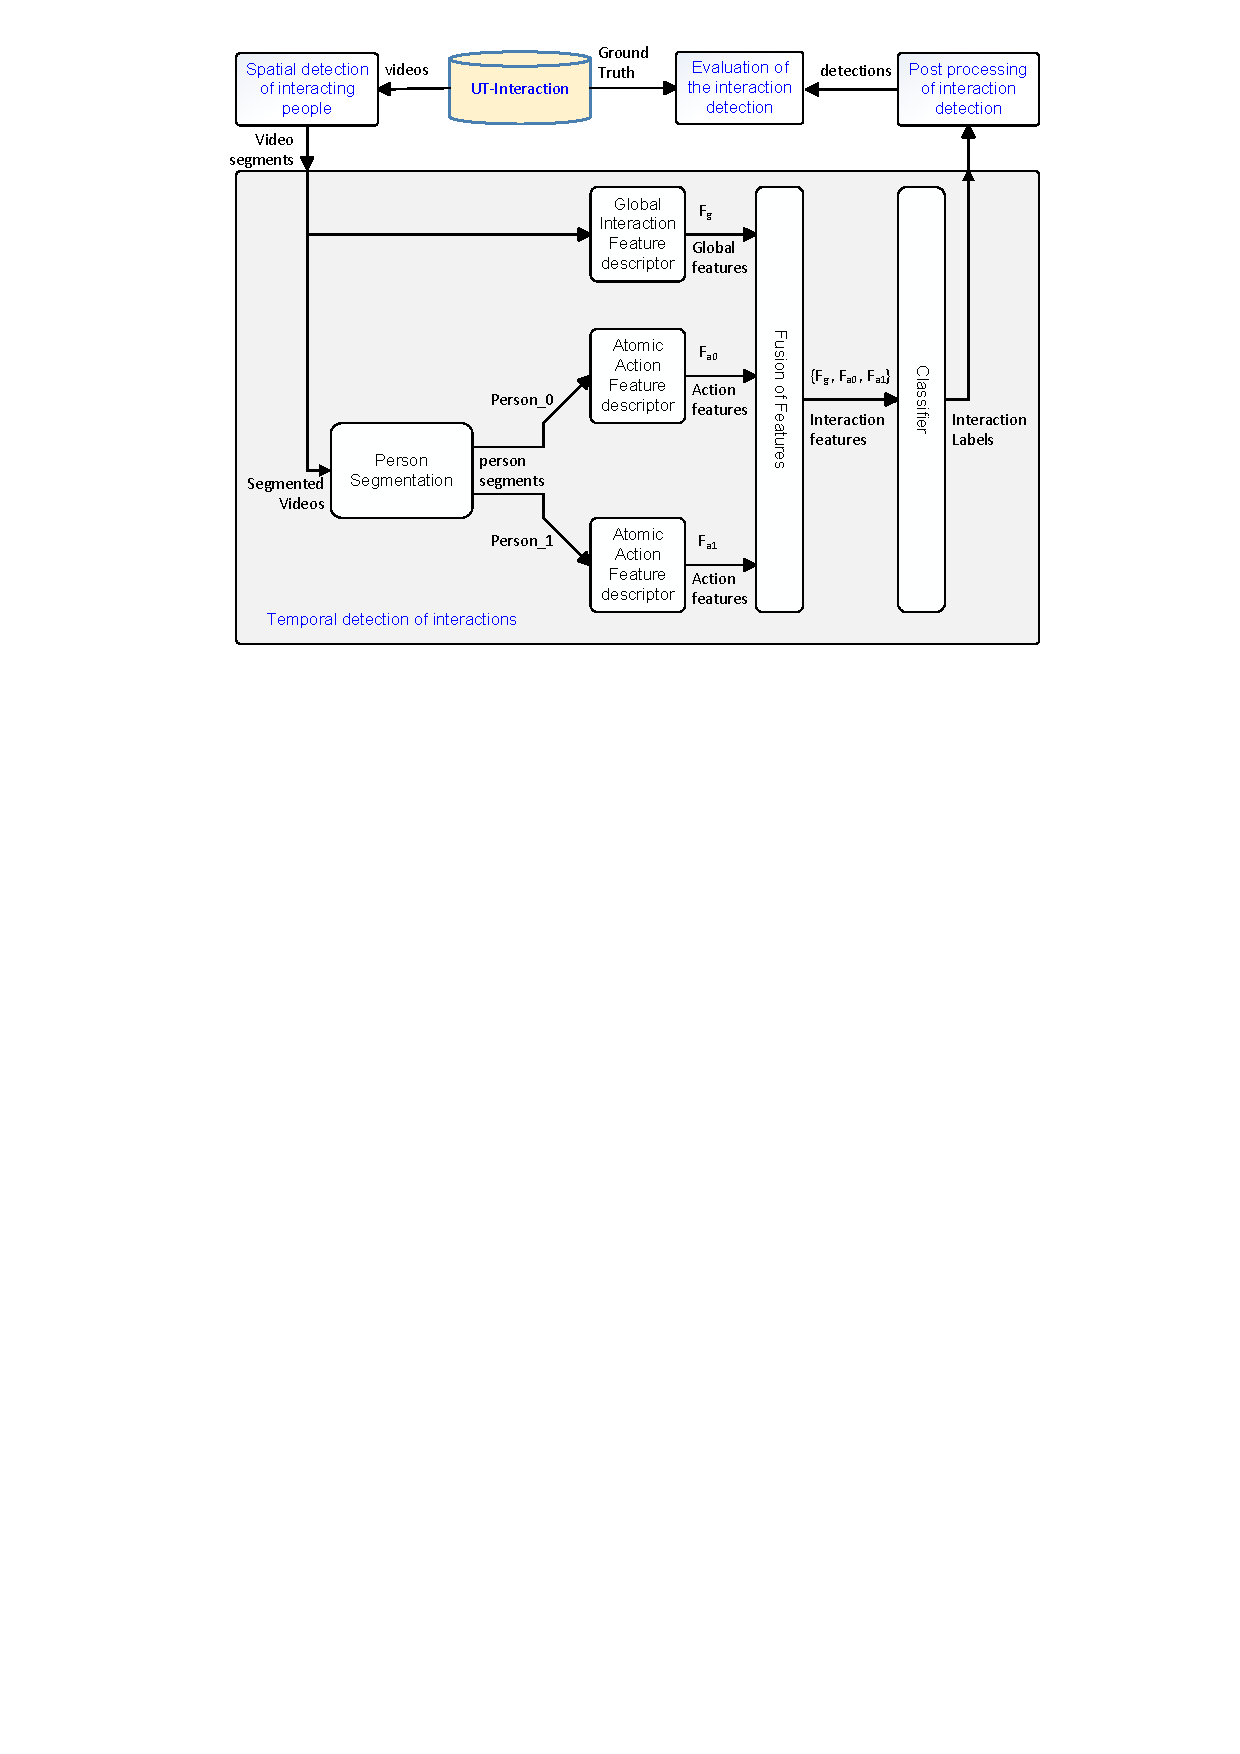
\includegraphics[trim=2.5cm 18.5cm 0cm 0.5cm]{fig01/arch_det.pdf}
	\caption{Overall framework of the interaction detection. }
	\label{fig:arch_det}
\end{figure}

\section{Models}
We introduce the main models employed in the interaction classification and detection. Since there are many model overlaps between interaction classification and detection, we introduce the main models in flat mode rather separately introduce them for classification and detection.   
\subsection{Person Segmentation}
\label{person_segmentation}
We locate the position of each person in each frame of the input videos, and track them throughout the video. Then we can use the bounding boxes of each person to split each input video into two video segments. The structure of the person segmentation is illustrated in Figure \ref{fig:person_detection}. There is no special challenges to perform person detection and tracking in the videos of UT-Interaction dataset because the background is relative simple and there is no much occlusions between people. So, for simplicity, we employ the classical Histogram of Oriented Gradients (HOG) feature descriptor plus a linear Support Vector Machines (SVM) framework to construct the person detector \cite{inria_person}.  Due to there may be some missing detections of one or two people in some frames, we employ the Kalman Filter to track each person throughout each video. Due to the fact that the relative position of the interacting people will be kept, i.e. if one of the interacting people first appear at left then he will kept at left in the whole video, we can simply match the interacting people according to their relative position. 
    
\begin{figure}
	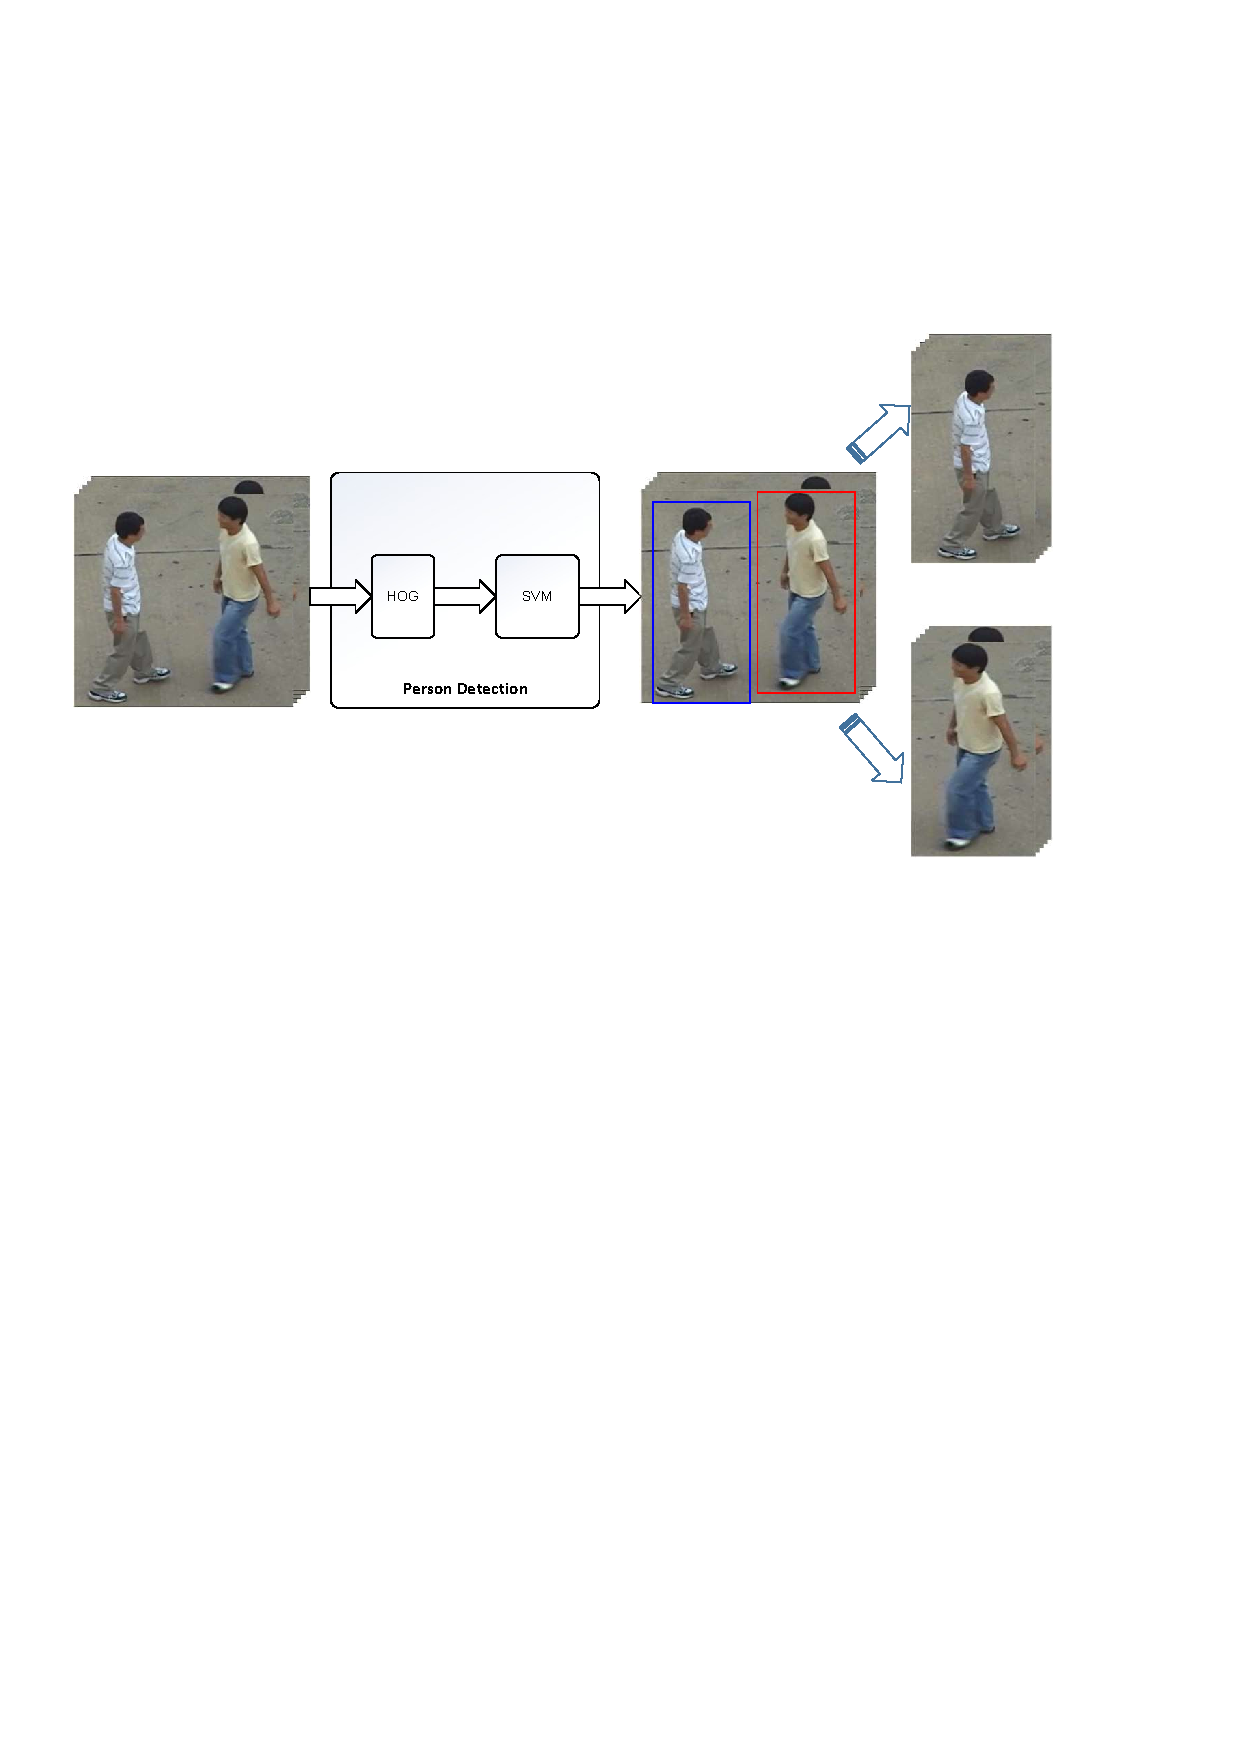
\includegraphics[trim=2cm 23cm 0cm 1cm]{fig01/person_detection.pdf}
	\caption{The architecture of the person segmentation}
	\label{fig:person_detection}
\end{figure}

\subsection{Spatial detection of interacting people}
For the interaction detection task, since there are both interacting and irrelevant people are present in the scene, we need to locate the positions for the interacting people and omit the irrelevant people. The overall architecture of the spatial detection of interacting people is illustrated in Figure \ref{fig:ip_det}. We adopt the same model to detect all people in each frame and to track interacting people as the person detection and tracking in the Section \ref{person_segmentation}. The only difference here is that we need the extra works to locate the interacting people and omit the irrelevant people which we will introduce in detail in the next chapter \ref{locate_interacting_people}.  
\begin{figure}
	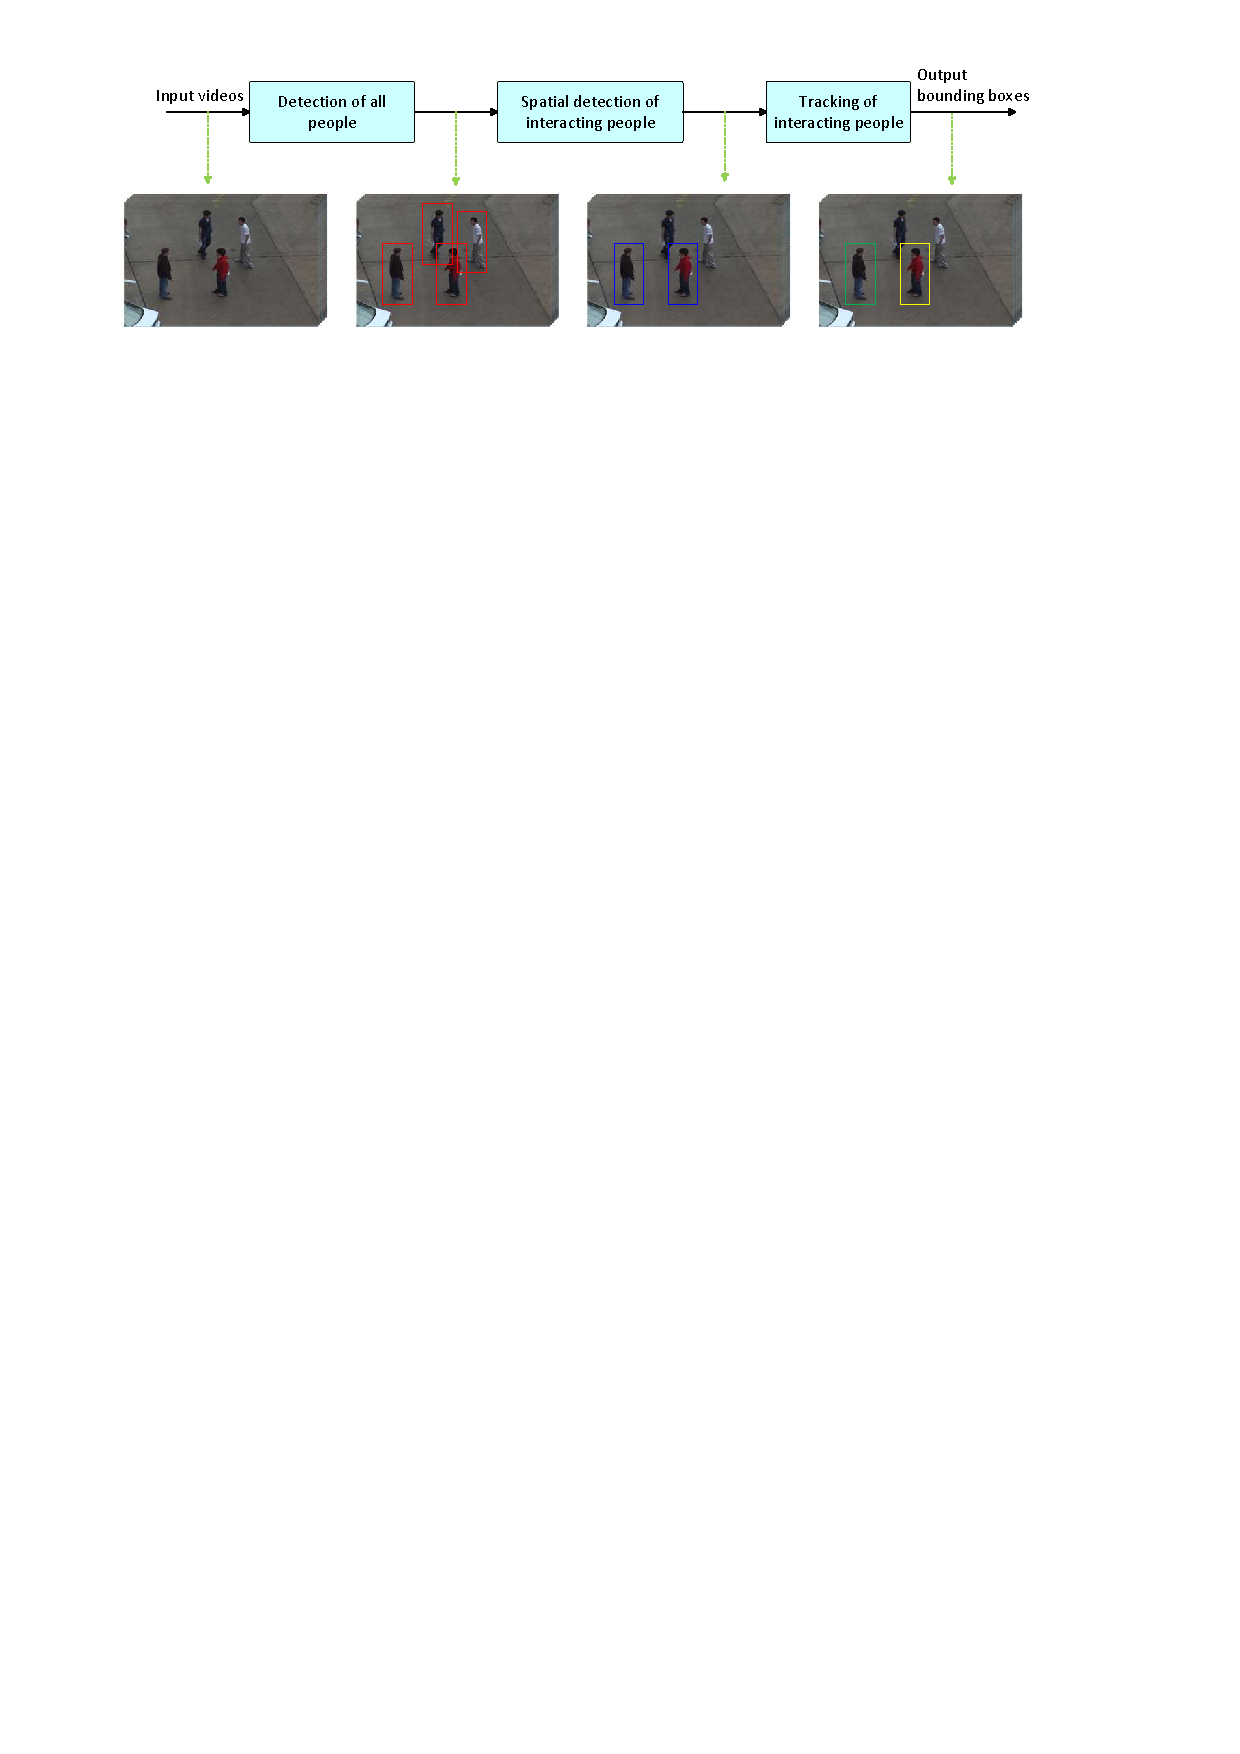
\includegraphics[trim=2cm 24cm 0cm 1cm]{fig01/ip_det.pdf}
	\caption{The architecture of the person segmentation}
	\label{fig:ip_det}
\end{figure}

\subsection{Feature Descriptor}
\label{3_3}
We employ the hierarchical feature descriptors, including a global feature descriptor which learns the global features, such as the relative position and orientation between two-person, and two atomic feature descriptors which learn the local atomic action features for each person. By doing this, our hierarchical feature descriptor is expected to learn both the hight-level complex interaction features and low-level detail atomic action features. The global feature descriptor and the atomic action feature descriptors share similar network frameworks. We use different network parameters between the global feature descriptor and the atomic feature descriptors. 
\par 
Our feature descriptors are all designed based on the 3D ConvNet \cite{Tran2015}. 3D ConvNet learns both spatial and temporal features at the same time by applying three-dimensional (x,y,time) convolution and pooling. The architecture of our 3D-ConvNet based feature descriptor is similar to  Tran et al.'s 3D-ConvNet\cite{Tran2015} . The architecture of our 3D-ConvNet is illustrated in Figure \ref{fig:c3d}. 
\begin{figure}
	\includegraphics[trim=2cm 26cm 0cm 0cm]{fig01/3dConvNet.pdf}
	\caption{Overall Architecture of the 3D-ConvNet. }
	\label{fig:c3d}
\end{figure}

\section{Training}
\label{3_4}
Since the performance of a learning algorithm is highly dependent on the training datasets, it is important to select proper training datasets for each network and balance the performance and computational complexity at the same time.
  
\subsection{Train the person detection network}
For simplicity, we directly use a pre-trained HOG plus linear SVM classifier trained on \textbf{INRIA Person Dataset} \cite{inria_person} as our person detector. The INRIA Person Dataset is one of the most used datasets for static people detection, which provides original images and the corresponding annotations. The training set contains 614 (2416 people) positive images and 1218 negative images.

\subsection{Train the feature descriptor}
There is an extra class for the interaction detection task because the video clips which contain no interaction need to be annotated an extra label. So, we train the feature descriptor for the interaction classification and the detection with different training set.

\subsubsection*{Train the feature descriptor for the interaction classification task } 
We adopt different training strategies between the global feature descriptor and atomic action feature descriptors. 
\par
For the global feature descriptor, we train it directly on the training data of the \textbf{UT-Interaction} dataset, see \ref{ut-interaction}. Before feeding training data to optimize the parameters, we first resize all segmented videos to \(128 \times 144 \) pixels; randomly sampling a \(112 \times 128 \) region; augment the training videos by horizontal flipping and multi-time random cropping; temporally down-sample the frames and finally split each input video into several 16-frame video clips with 8 frames overlap. We use the adaptive moment estimation (ADAM) to optimize our models. We use mini-batch of 16 examples (video clips) and initial learning rate of \(1e^(-4)\) which is further divided by 2 for every 4 training epochs.  
\par
For the atomic action feature descriptors, we will test both the pre-training plus fine-tuning strategy and the directly training strategy. Since we have large scale single person action datasets available, we will observe whether the pre-trained network can further improve the performance. For the pre-training plus fine-tuning strategy, large scale action video dataset \textbf{UCF-101} \cite{ucf101} will be used to pre-train the atomic action feature descriptor and the video segments generated by the person segmentation, see \ref{person_segmentation}, will be used to fine-tune it. For the directly training strategy, we train the network directly on the video segments generated by the person segmentation.  We adopt the same method of augmentation and pre-processing which we have applied to train the global feature descriptor except that the final resolution of the video clips is \(112 \times 80\) instead of \(112 \times 128\).  The method of optimization is also as same as that of the global feature descriptor. 

\subsubsection*{Train the feature descriptor for the interaction detection task }
We adopt the same strategy as the classification task to train the feature descriptor for the detection task except that the some negative training videos are added to the training set and there are 7 class labels instead of 6. Those negative training videos are generated by randomly cropping in the unsegmented videos, see \ref{ut-interaction}, and for each that does not overlap with any positive bounding boxes, see \ref{extra_class} for detail.

 
\subsection{Train the Classifier}
All the output features of the global feature descriptor \(F_g\) and the atomic action feature descriptors \(F_{a0}\) and \(F_{a1}\) are concatenated as \{\(F_g, F_{a0}, F_{a1}\)\} and fed to the softmax classifier. These features are extract from the target dataset \textbf{UT-Interaction}.  
%=========================================================